%%%%%%%%%%%%%%%%%%%%%%%%%%%%%%%%%%%%%%%%%%%%%%%%%%%%%%%%%%%%%%%%%%%%%%
% LaTeX Example: Project Report
%
% Source: http://www.howtotex.com
%
% Feel free to distribute this example, but please keep the referral
% to howtotex.com
% Date: March 2011 
% 
%%%%%%%%%%%%%%%%%%%%%%%%%%%%%%%%%%%%%%%%%%%%%%%%%%%%%%%%%%%%%%%%%%%%%%
% How to use writeLaTeX: 
%
% You edit the source code here on the left, and the preview on the
% right shows you the result within a few seconds.
%
% Bookmark this page and share the URL with your co-authors. They can
% edit at the same time!
%
% You can upload figures, bibliographies, custom classes and
% styles using the files menu.
%
% If you're new to LaTeX, the wikibook is a great place to start:
% http://en.wikibooks.org/wiki/LaTeX
%
%%%%%%%%%%%%%%%%%%%%%%%%%%%%%%%%%%%%%%%%%%%%%%%%%%%%%%%%%%%%%%%%%%%%%%
% Edit the title below to update the display in My Documents
%\title{Project Report}
%
%%% Preamble
\documentclass[paper=a4, fontsize=11pt]{scrartcl}
\usepackage[T1]{fontenc}
\usepackage{fourier}
\usepackage{natbib}
\usepackage[english]{babel}															% English language/hyphenation
\usepackage[protrusion=true,expansion=true]{microtype}	
\usepackage{amsmath,amsfonts,amsthm} % Math packages
\usepackage[pdftex]{graphicx}	
\usepackage{url}
\usepackage{multirow}
\usepackage{array}

%%% Custom sectioning
\usepackage{sectsty}
\allsectionsfont{\centering \normalfont\scshape}


%%% Custom headers/footers (fancyhdr package)
\usepackage{fancyhdr}
\pagestyle{fancyplain}
\fancyhead{}											% No page header
\fancyfoot[L]{}											% Empty 
\fancyfoot[C]{}											% Empty
\fancyfoot[R]{\thepage}									% Pagenumbering
\renewcommand{\headrulewidth}{0pt}			% Remove header underlines
\renewcommand{\footrulewidth}{0pt}				% Remove footer underlines
\setlength{\headheight}{13.6pt}


%%% Equation and float numbering
\numberwithin{equation}{section}		% Equationnumbering: section.eq#
\numberwithin{figure}{section}			% Figurenumbering: section.fig#
\numberwithin{table}{section}				% Tablenumbering: section.tab#


%%% Maketitle metadata
\newcommand{\horrule}[1]{\rule{\linewidth}{#1}} 	% Horizontal rule

\title{
		%\vspace{-1in} 	
		\usefont{OT1}{bch}{b}{n}
		\normalfont \normalsize \textsc{CSE 582 Final Project Report} \\ [25pt]
		\horrule{0.5pt} \\[0.4cm]
		\huge Generating Targeted Novelty Questions with AskMeAnything QA Session Data \\
		\horrule{2pt} \\[0.5cm]
}
\author{
		\normalfont 								\normalsize
        Ehsanul Kabir\\[-3pt]		\normalsize
        \today
}
\date{}


%%% Begin document
\begin{document}
\maketitle
\section{Introduction}
Automatic question generation is a fascinating and vital aspect of natural language processing, which holds the potential to revolutionize fields such as education, information retrieval, and question answering systems. In this particular project, I am dedicated to developing a method for generating unique and targeted questions that focus on a specific topic and context. These questions should also pertain to the questionee's knowledge or experiences that aren't covered in the provided context or aren't common knowledge about the individual. I refer to these types of questions as "novelty questions" as they spark curiosity and provide deeper insights.

For this project, I decided to harness the power of the IAmA subreddit's AskMeAnything (AMA) sessions. AMA sessions are a treasure trove of information, presenting a rich variety of topics and contexts to explore. People from diverse backgrounds participate in these sessions, answering questions from the Reddit community about their personal experiences, expertise, or unique perspectives. This dataset provides an excellent opportunity to create and refine a model that generates novelty questions that are both engaging and relevant.

To achieve this goal, I employed a two-step approach. First, I trained a T5 seq2seq model on the AMA dataset. The T5 model is known for its strong performance in various natural language processing tasks, and by fine-tuning it on the AMA data, it would ideally be able to generate novelty questions that are coherent, contextually relevant, and interesting.

However, I wanted to take this project a step further by filtering out questions that might not be as relevant to the context. To accomplish this, I fine-tuned a BERT model on the AMA data as well, which served as a ranking mechanism. The BERT model assessed the generated questions based on their relevance to the context, ensuring that only the most appropriate and intriguing questions made it through the filtering process.

Once the models were trained and the question generation process was established, it was time to evaluate the effectiveness of the generated novelty questions. To do this, I used several well-known evaluation metrics, such as BLEU, ROUGE, and METEOR. These metrics helped me gauge the quality, relevance, and novelty of the generated questions in a quantitative manner. In addition to these metrics, I also conducted a human evaluation, seeking input from real people to assess whether the questions were engaging, contextually relevant, and genuinely novel.

In summary, this project is dedicated to generating novelty questions on specific topics and contexts using a T5 seq2seq model trained on IAmA subreddit's AMA sessions.\footnote{\url{https://www.reddit.com/r/IAmA/}} Furthermore, a fine-tuned BERT model is employed to rank and filter out questions based on their contextual relevance. The generated questions are evaluated using a combination of standard metrics and human evaluation, ensuring that the questions are both engaging and insightful. The trained question generator is available as a web application at HuggingFace\footnote{\url{https://huggingface.co/spaces/ehsanul007/IAmA-question-generator}} and can be accessed by anyone. 
The datasets are alsox available at HuggingFace\footnote{Question Generation Dataset: \url{https://huggingface.co/datasets/ehsanul007/IAmA-question-generator} \\ Question Ranking Dataset: \url{https://huggingface.co/datasets/ehsanul007/IAmA-question-ranking}} and can be accessed by anyone.

\section{Data Collection and Preprocessing}
% create a new table
\begin{table}
\centering
\scriptsize
\begin{tabular}{lm{2.5cm}m{2.5cm}m{2.5cm}m{2.5cm}}
  \hline
   & \multicolumn{4}{c}{\textbf{IAmA Subreddit Original Post Titles}} \\
  \cline{2-5}
   & I am  \textbf{Jason Steele}, creator of Charlie the Unicorn, Llamas with Hats, and other internet videos. Ask me anything! & I'm a retired  \textbf{bank robber}. AMA! & I’m  \textbf{Lynda Carter}, Wonder Woman actress and singer. Ask Me Anything! & Sup muthafuckas!  \textbf{Ron Perlman} here. Don’t be shy- Ask Me Anything! \\
   \cline{2-5}
   \cline{2-5}
    & What caused you to take the Llamas with Hats series in the direction that you did, from hilariously morbid to actually somewhat sad? & You say that you're retired. But I know a guy who is looking to put together a crew for a major job. This is the one you've been dreaming of all these years. Are you up for one last job? & Hello! Thanks for doing this AMA. Were you ever asked to reprise your role as Wonder Woman for another show, even a cameo? & Why doesn't anybody ever bring up how fucking great City of Lost Children was? \\
   \cline{2-5}
   \textbf{Comments} & Hi there! What was your inspiration for Charlie the Unicorn? & How many pounds of shit, would you say, were in your pants while walking out the door? & Thank you for doing this AMA. I just wanted to know, how did it feel, starring on modern superhero shows like Smallville and Supergirl, as opposed to the Wonder Woman show of the 70's? & Now that photos have been released, how do you feel about the 'new' Hellboy? \\
    \cline{2-5}
   & How does it feel having created some of the most memorable animations on the Internet?  & "Why, is that mister Clay coming in with the gun? Well, goshdarnit, is it thursday already?" & Hi Lynda! Thanks for doing this AMA! How did you like working on Fallout 4? Magnolia was such a great character! & Who would you want to play you in a Sons of Anarchy prequel? \\
  \hline
  \hline
  \end{tabular}
  \caption{Sample of AMA post and questions}
  \label{tab:ama_sample}
\end{table}

I chose to use the IAmA subreddit's AskMeAnything (AMA) sessions as my primary source of context and questions. To collect the data, I utilized both the PRAW and PMAW Python libraries, which made the process much smoother. I decided to focus on AMA sessions from the years 2014 to 2021 for a comprehensive dataset.

During this time period, there were a total of $498$ AMA sessions that garnered more than $1000$ level-0 comments each. Level-0 comments are those that appear directly beneath the original post and are highly likely to be questions aimed at the original poster. I opted for a cutoff of $1000$ comments to ensure that the dataset would primarily consist of popular AMA sessions. However, some popular AMA request posts still slipped through the cracks and needed to be filtered out afterward.

I then split the dataset, selecting sessions from $2015$ to $2021$ for training and validation purposes, while using the $2014$ sessions as the test set. To further refine the data and reduce the training set size, I applied additional selection criteria to the comments. For each AMA session, I kept only level-0 comments with at least $10$ upvotes, which helped to highlight better-quality comments.

After applying these selection criteria, I ended up with a total of $22,246$ AMA questions, along with their respective original posts as context. The test set contained $2284$ questions, while the training and validation sets each comprised $11,123$ questions.
Table \ref{tab:ama_sample} shows a sample of the collected data.

\subsection*{Adding Topic}
% create a new table
\begin{table}
\centering
\scriptsize
% \begin{tabular}{p{6cm}p{3cm}}
\begin{tabular}{m{6cm}m{3cm}}
  \hline
  \textbf{Question} & \textbf{Topic} \\
  \hline
  \hline
  Hello! Thanks for doing this AMA. Were you ever asked to reprise your role as Wonder Woman for another show, even a cameo? &  Wonder Woman reprisal \\
  \hline
Thank you for doing this AMA. I just wanted to know, how did it feel, starring on modern superhero shows like Smallville and Supergirl, as opposed to the Wonder Woman show of the 70's? &  Acting in superhero shows \\
\hline
Hi Lynda! Thanks for doing this AMA! How did you like working on Fallout 4? Magnolia was such a great character! &  Fallout 4 and Magnolia \\
\hline
Hi, I just want to know one thing. Where did you park your plane? &  Airplane Parking \\
\hline
What was your most funny moment behind the scenes of Wonder woman? &  Funny moments behind the scenes \\
  \hline
  \hline
  \end{tabular}
  \caption{Sample of generated topics using GPT3 API}
  \label{tab:topic_sample}
\end{table}

The topic of each question is not explicitly stated in the context. Nevertheless, it can often be deduced from the question itself. Manually annotating the topic for every question would be a time-consuming process, so I opted to use the GPT-3 API to generate the topics instead.

To do this, I employed the following prompt: \textit{Describe the topic of the question below in a single word/phrase. Q: <question> A: ?}. This prompt allowed GPT-3 to generate a topic based on the input question. Table \ref{tab:topic_sample} presents a sample of the topics produced by the API. As we can see from this sample, the generated topics are relevant and closely related to the questions themselves.


\subsection*{Padding Context with Wikipedia Summary}
\begin{table}
\centering
\tiny
\begin{tabular}{p{5cm}p{5cm}}
  \hline
  \textbf{Title} & \textbf{Summary} \\
  \hline
  \hline
  Hello, I'm Lorin. I make music called Bassnectar - lately i've been working nonstop to remix my record collection into new versions for an experiment called the Freestyle Sessions in Colorado! What's on your mind? An me askything... & Lorin Gabriel Ashton, better known under his stage name Bassnectar (born February 16, 1978), is an American DJ and record producer. \\
  \hline
  I Work at a Costco in Oregon dealing with this corona virus craze, AMA! & Costco Wholesale Corporation (doing business as Costco Wholesale and also known simply as Costco) is an American multinational corporation which operates a chain of membership-only big-box retail stores (warehouse club). As of 2022, Costco is the fifth largest retailer in the world and is the world's largest retailer of choice and prime beef, organic foods, rotisserie chicken, and wine as of 2016. \\
  \hline
  I’m a 23 year old woman living with Addison’s Disease, Lupus, Psoriasis and Psoriatic Arthritis. Basically a walking autoimmune disease. Ask me anything! & Addison's disease, also known as primary adrenal insufficiency, is a rare long-term endocrine disorder characterized by inadequate production of the steroid hormones cortisol and aldosterone by the two outer layers of the cells of the adrenal glands (adrenal cortex), causing adrenal insufficiency. Symptoms generally come on slowly and insidiously and may include abdominal pain and gastrointestinal abnormalities, weakness, and weight loss. \\
  \hline
  Hey Reddit, it’s Kris, Rob and Dave from Cyanide \& Happiness! Let’s talk about things! & Cyanide \& Happiness (C\&H) is a webcomic created by Rob DenBleyker, Kris Wilson, Dave McElfatrick and Matt Melvin. The comic has been running since 2005 and is published on the website explosm.net along with animated shorts in the same style. Matt Melvin left C\&H in 2014, and several other people have contributed to the comic and to the animated shorts.  \\
  \hline
  \hline
  \end{tabular}
  \caption{Sample of appended context from Wikipedia}
  \label{tab:wiki_sample}
\end{table}
AMA posts are composed of a title and a body. The title serves as a brief introduction to the questionee or the original poster (OP). However, in many cases, the titles proved to be too short to provide adequate context for the model. For instance, famous TV or movie actors and actresses often simply included their name in the title, which was enough for readers to identify them but insufficient for the model to learn the context. Furthermore, the post body usually didn't contain much relevant information.

Consequently, it became necessary to append additional context from named entities to the original post. Automating this task was quite challenging, as the questionees ranged from celebrities to various organizations. Titles frequently featured multiple entities, and including context for all of them would overload the model. Thus, I manually selected a single main entity from each title, ensuring that the entity had a Wikipedia page.

Occasionally, the OP was not a well-known figure or organization and didn't have a Wikipedia page. In these cases, the OP typically provided enough information about themselves in the title. For titles containing at least one notable entity, I employed the Wikipedia API to retrieve summaries from the entity's Wikipedia page. Since the summaries varied in length, I chose a sufficient number of sentences to achieve a total of $50$ tokens in each summary.

I then appended these summaries to the original post title, which served as the context for the questions. For questionees without a Wikipedia page, I used the original post title as context. Table \ref{tab:wiki_sample} displays a sample of the generated summaries. As we can see from these samples, the summaries are relevant to the title and blend seamlessly into the appended context.


\subsection*{Additional Pre-processing of Title}
The titles contained a lot of special characters and emojis.
They also contained a lot of variations of the text `Ask Me Anything' which needed to be filtered.
I used various regular expressions to filter out the special characters and emojis along with the variations of `Ask Me Anything'.


\subsection*{Qualitative Analysis of Data}
The above selection criteria and pre-processing steps helped clean the data to a great extent.
Specifically, I did not notice any post among the selected posts that were not an AMA session.
However, there were some questions that seemed to be more of a comment than a question and some questions that seemed like a follow-up question.
I did not remove those questions as they were not a significant portion of the data and the task of identifying them would be challenging and out-of-scope for this project.

Below I have listed some issues with the data that could not be solved within the limited time frame of this project:
\begin{itemize}
  \item Some reddit questions were informal and contained a lot of abbreviations and slang. (Not necessarily an issue but could be a challenge for the model to learn)
  \item Some questions were actually comments or follow-up questions which is not expected from a question generator model without knowledge of the prior conversation.
  \item The appended context could not be expected to cover all the information about the questionee and as a result, some questions are relevant to the questionee but it is not obvious from the context. The model would need more familiarity with the questionee to be expected to generate such questions which may only be possible with a large LLM model like GPT-3 or GPT-4.
  \item The AMA sessions were from a few years back but the appended context was from the current Wikipedia page of the questionee. This could be an issue for the model to learn the context.
\end{itemize}

\subsection*{Quantitative Analysis of Data}
\begin{table}[h]
  \small
  \centering
  \begin{tabular}{lrrrr}
    \hline
     & mean & min & max & std \\
    \hline
    Context & 68.63 & 23 & 132 & 17.86 \\
    Question & 18.20 & 1 & 48 & 10.18 \\
    Topic & 2.61 & 1 & 5 & 0.95 \\
    \hline
    \end{tabular}
    \caption{Word count statistics of the data}
    \label{tab:data_stats}
\end{table}

I have listed some statistics about the data below:
\begin{itemize}
  \item Among the $22,246$ posts, there are $14,313$ unique topics. Top 5 most frequent topics are: Time Management, Clarification, Confusion, Identity verification, Miscommunication.
  \item The number of unique questionees is $16027$. Top 3 most frequent questionees are: \textit{'What is your favorite dinosaur?'}asked 4 times, \textit{'What is your favorite flavor of ice cream?'} and \textit{'Is a hotdog a sandwich?'} asked 3 times each.
  \item Of $428$ questionees, $134$ of them were random/anonymous persons hosting the AMA session with title hooks such as \textit{'I am a retired bank robber, AMA!'}.
  \item $24$ of the host reappeared in multiple AMA sessions.
  \item Table \ref{tab:data_stats} shows the word count statistics of the data.
\end{itemize}

\section{Methodology}

% force figure to be placed at the top of the page and start after the previous text
\begin{figure*}[t]
  \centering
  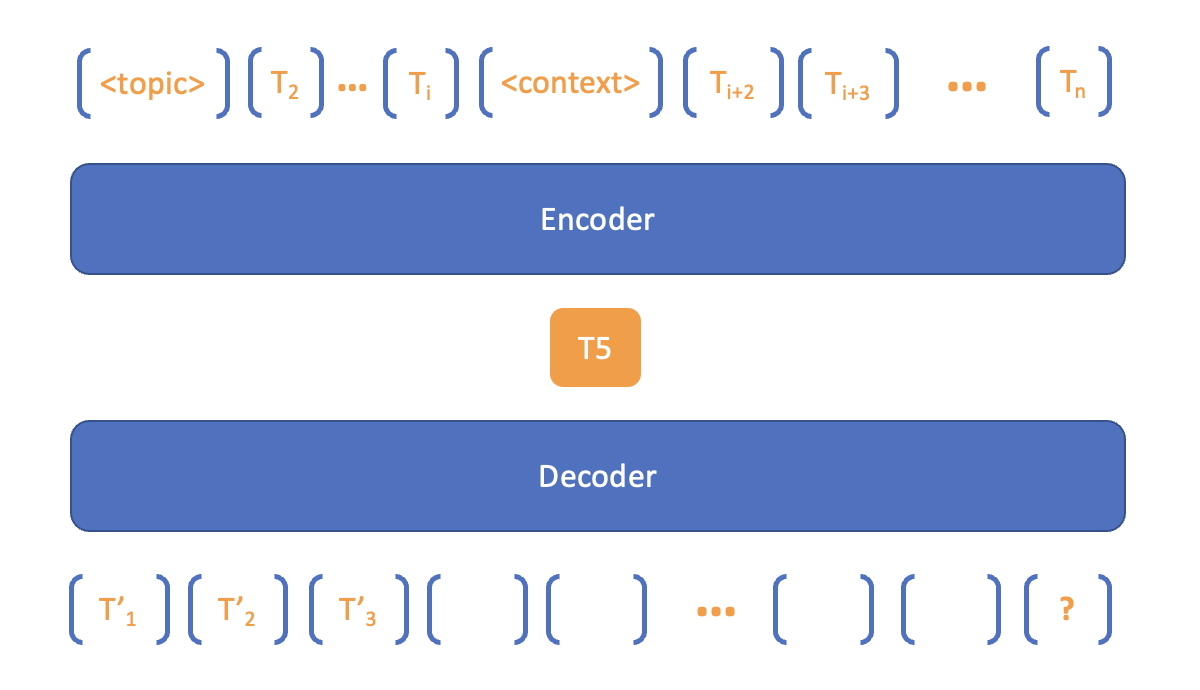
\includegraphics[width=0.6\textwidth]{t5.png}
  \caption{Question Generator Architecture}
  \label{fig:question_generator}
\end{figure*}


For the task of question generation, I used one question generator model and one question ranker model. 
The question generator model's goal is to generate as many well-constructed questions as possible on the given topic to the questionee.
The question ranker model's goal is to rank the generated questions based on their quality.
Afterwards, the top ranked question is selected as the final output.

\subsection{Question Generator}
The following steps were taken to train the question generator model:
\begin{itemize}
  \item The T5 seq2seq Transformer \cite{raffel2020exploring} was picked as the architecture for the question generator model.
  \item I picked a pre-trained T5 model from HuggingFace's model hub which was trained on an accumulation of various well-known QA datasets (SQuAD \cite{rajpurkar2016squad}, RACE \cite{lai2017race}, CoQA \cite{reddy2019coqa}, and MSMARCO \cite{nguyen2016ms}).
  \item The pre-trained model was fine-tuned on the AMA dataset that I prepared above.
  \item The fine-tuning is implemented as a conditional generation (seq2seq) task that maximizes the log-likelihood of the target sequence given the source sequence.
  \item The source sequence is a <topic> token followed by the topic of the question followed by a <context> token followed by the context of the questionee. The <topic> and <context> tokens are used to help the model learn the boundaries of the topic and the context and they were added to the original T5 tokenizer's vocabulary.
  \item The target sequence is the question asked by the reddit user on the given topic to the questionee.
\end{itemize}

\subsection{Question Ranker}
The following steps were taken to train the question ranker model:
\begin{itemize}
  \item The BERT Transformer \cite{devlin2018bert} was picked as the architecture for the question ranker model.
  \item The Transformer was fine-tuned on the AMA ranking dataset of positive and negative examples that I mentioned above.
  \item The fine-tuning is implemented as a binary classification task that maximizes the log-likelihood of the target label given the source sequence.
  \item The source sequence is the question and the context separated by <sep> token and the target label is 1 if the question is a relevant question to be asked to the questionee and 0 otherwise.
\end{itemize}

\section{Experiments}
\subsection*{Decoding Method}
Selecting the right decoding method is critical to ensure good output quality of the question generator model.
Beam search and nucleus sampling are two popular decoding methods for Transformer models to generate questions.
Nucleus sampling is a stochastic decoding method that samples from the smallest possible set of words whose cumulative probability exceeds a threshold $p$.
Since AMA questions are typically elaborate and long, I used beam search in my experiments.
The hyperparameters picked for beam search are as follows:

% decrease the space between items
\begin{itemize}
  \setlength\itemsep{0.1em}
  \small
  \item Number of beams: 20
  \item Number of beam groups: 10
  \item Maximum length of the generated question: 50
  \item Number of question candidates to generate: 5
  \item Diversity penalty: 0.5 (to encourage diversity among the generated questions)
\end{itemize}

\subsection*{Evaluation Metrics}
Qustion Generation task shares similarity with the summarization task and as such, the same evaluation metrics (ROUGE \cite{lin2004rouge}, BLEU \cite{papineni2002bleu}, METEOR \cite{banerjee2005meteor}, etc.) are typically used to evaluate the quality of the generated questions.
However, \cite{novikova2017we} showed that the standard evaluation metrics are not suitable for evaluating the quality of NLG tasks such as question generation.
%Therefore, in addition to the standard evaluation metrics, I use the BLEURT \cite{sellam2020bleurt} metric which is state-of-the-art evaluation metric in WMT Metrics shared task.
Therefore, manual evaluation is necessary to evaluate the quality of the generated questions.
There was no baselines considered for this project considering the limited time and resources.


\subsection*{Hyperparameters}
The hyperparameters used for the question generator model are as follows:

\begin{table}
  \tiny
  \centering
  \begin{tabular}{lrr}
    \hline
    \textbf{Hyperparameter} & \textbf{Question Generator} & \textbf{Question Ranker} \\
    \hline
    Batch size & $8$ & $64$ \\
    Learning rate & $0.0001$ & $0.0001$ \\
    Number of epochs & $20$ & $20$ \\
    \hline
  \end{tabular}
  \caption{Training Hyperparameters}
  \label{tab:hyperparams_qg}
\end{table}

Both model was trained on a single NVIDIA A100 GPU.
The code was written in a combination of PyToch and HuggingFace's Transformers library.
Code from the github repository \url{https://github.com/AMontgomerie/question_generator.git} was used as a reference for the implementation of the question generator and the question ranker models.
The generator model was trained for $20$ epochs and took about $6$ hours to train.
The ranker model was trained for $20$ epochs and took about $1$ hours to train.
The trained question generator model is available at HuggingFace\footnote{\url{https://huggingface.co/ehsanul007/IAmA-question-generator}} and the trained question ranker model is available at HuggingFace\footnote{\url{https://huggingface.co/ehsanul007/IAmA-question-ranker}}.


\section{Results and Analysis}

\subsection*{Automatic Evaluation}

\begin{table}
  \footnotesize
  \centering
  \begin{tabular}{lrrrrrr}
    \hline
    Test Set & BLEU-1 & BLEU-2 & BLEU-3 & BLEU-4 & METEOR & ROUGE \\
    \hline
    Familiar Questionee & $16.47$ & $6.26$ & $3.82$ & $2.82$ & $15.68$ & $13.57$ \\
    Unfamiliar Questionee & $17.24$ & $7.20$ & $4.45$ & $3.26$ & $16.73$ & $14.02$ \\
    \hline
  \end{tabular}
  \caption{Performance of the question generator model on the familiar and unfamiliar questionee test sets. (The scores are in percentage. BLEU-1, BLEU-2, BLEU-3, BLEU-4 refer to BLEU scores for n-grams of length 1, 2, 3, 4 respectively.)}
  \label{tab:qg_results}
\end{table}

Two test sets were considered in automatic evaluation of the question generator model.
The unfamiliar questionee test set consists of questions asked by reddit users to questionees that were not present in the training set i.e. from the AMA sessions in 2014.
The familiar questionee test set consists of questions asked by reddit users to questionees that were present in the training set and they were randomly sampled from the validation set.
The motivation behind using two test sets is to evaluate the generalization ability of the question generator model and whether it is affected by exposure to the questionee context during training.

Table $\ref{tab:qg_results}$ shows the evaluation metrics for the question generator model on the familiar and unfamiliar questionee test sets. 
The performance of the question generator model is slightly better on the unfamiliar questionee test set than the familiar questionee test set.
However, the difference is negligible.
One explanation for this is that the context available to the question generator model is not sufficient to generate inference capability about the questionee which could have helped the model to generate better questions.
Thus, the model tries to generate similar questions for the same questionee to what it has seen during training even though topics are different.
However, the above is just a hypothesis and further investigation is required to confirm it.
Overall, the automatic evaluation results show that the question generator model is not able to generate questions that are similar to the questions asked by reddit users in the AMA sessions.

\subsection*{Human Evaluation}
\begin{table}
  \small
  \centering
  \begin{tabular}{p{2cm}p{2cm}p{2cm}p{2cm}}
    \hline
    \textbf{Semantic Similarity with Actual Question} &	\textbf{Grammatical Correctness} &	\textbf{Degree of Novelty} &	\textbf{Relevance to Questionee} \\
    \hline
    0.83 &	2.5	& 2.1 &	1.37 \\
    \hline
  \end{tabular}
  \caption{Human evaluation results for the generated questions. (The scores are out of 3)}
  \label{tab:human_eval}
\end{table}

Table $\ref{tab:human_eval}$ shows the results of the human evaluation of the generated questions on various aspects.
As this was a one-person project, the human evaluation was done by the author of this report.
The human evaluation was done on a sample of $100$ generated questions.

The results show that the generated questions are not semantically similar to the actual questions asked by reddit users in the AMA sessions.
However, that is neither surprise nor unwelcome in this case.
Novelty questions are not expected to be semantically similar to the actual questions.

The generated questions have a high degree of grammatical correctness.
This is impressive considering that the questions generated by the question generator model are long and complex.

The generated questions have a high degree of novelty evaluated by the human evaluator.
This means that the goal of generating novel questions is moderately achieved.
However, the generated questions are not relevant to the questionee.
The novelty comes at the cost of losing connection with the context.

\subsection*{Case Study}
\begin{table}
  \tiny
  \centering
  \begin{tabular}{p{1cm}m{2.5cm}m{2.5cm}m{2.5cm}m{2.5cm}}
    \hline
    \textbf{Questionee Context} & \textbf{Topic} & \textbf{Context} & \textbf{Actual Question} & \textbf{Generated Question} \\
    \hline
    \hline
    Familiar & Work experiences & I am a Video and Audio Forensic Expert who has consulted on cases like Trayvon Martin, Malaysia Airlines Flight 307, and the JFK Tapes! & In your 34 years of work, what it the weirdest or strangest thing you learned in your time? & What is the \textbf{craziest} thing to ever happened to your job? \\
    \hline
    Familiar & Inter-coastal &	We are the staff of Giant Bomb, a site about video games, and our decades of video game coverage experience are here to serve you today. \textit{Giant Bomb is an American video game website and wiki that includes personality-driven gaming videos, commentary, news, and reviews, created by former GameSpot editors \textbf{Jeff} Gerstmann and Ryan Davis. The website was voted by Time magazine as one of the Top 50 websites of 2011.}	& With how busy you guys are on different coasts, how much content on the site that you're not directly involved in do you consume?  For example, do you listen to each others podcasts? & Jeff, what are your thoughts on intercoastal waters? \\
    \hline
    Familiar & Movie Rankings/Voting & We are Jeremy \& Barrett of CinemaSins, MusicVideoSins, \& the SinCast podcast./AMA  & Once you've reached 2016 on SinCast, will you continue to vote on your favourite movies for each year? What other topics do you have planned for then? & What's your favorite topic of movies that you have discussed on the \textbf{Sincast}? And which movie(s) that you have mentioned that you have the most fun times watching? Also, which movies/shows are you watching should \\
    \hline
    Familiar & Unconventional viewing habits & We are the Pornhub team. & Odd? I browse Pornhub exclusively for the Halo montages! & What is the \textbf{craziest} thing you've seen someone do on \textbf{Pornhub}? \\
    \hline
    Familiar &  Clothing style comparison. & Hi, Im Hiroshi Lockheimer, here at Google with the team that build Nexus 5X \& 6P. & Who wins the best shirt award on the Android team? Matias Duarte with his colorful dress shirts or Dave Burke with his graphic Ts? & How does the Nexus 6P differ from the other android 6P? \\
    \hline
   Unfamiliar & Opinion of Victoria & I am Cyndi Lauper. Whaddya wanna know? & Is Victoria really as cool as everyone says she is? & What do you really think of Victoria? \\
    \hline
   Unfamiliar & Actor Collaboration & I am Cyndi Lauper. Whaddya wanna know?  & Was it more fun to work with Christopher Walken, or Paul Rubens? & Who was your \textbf{favorite} actor to work with? \\
   \hline
   \end{tabular}
  \caption{Examples of generated questions by the question generator model. Appended context is omitted for brevity unless it is necessary to understand the question.}
  \label{tab:qg_examples}
\end{table}

Table $\ref{tab:qg_examples}$ shows some examples of generated questions by the question generator model.
Some interesting observations are listed below:
\begin{itemize}
  \item The generated question likes to \textit{address the questionee by name}. Example 2 shows one interesting such case where an inference is made about the questionee's name.
  \item Except few patterns such as finding the name of the questionee, not much attempt is made to infer about the questionee. The evidence of this is the fact that \textit{most questions could be generated by looking at the topic alone}. Not much information about the questionee is integrated into the generated question.
  \item The effort to generate an interesting/novel question is evident in the generated questions. Instead of asking dull factoid questions, the generated \textit{questions are more opinionated and eager to use superlatives} such as \textit{best}, \textit{craziest}, \textit{favorite} etc.
  \item If there are multiple words in the topic, the \textit{words that are not relevant to the questionee are ignored}. In example 5, the topic is \textit{Clothing style comparison}. The words \textit{Clothing style} are not relevant to the questionee. So, the generated question is about the word \textit{comparison}. This observation is in contrast to the observation made in the second bullet point. 
  \item No difference is visible in the generated questions when the questionee is familiar or unfamiliar to the question generator model.
  \end{itemize}

\subsection*{Topic Dependency of Generated Questions}
\begin{table}
  \tiny
  \centering
  \begin{tabular}{m{1.5cm}m{3.5cm}m{3.5cm}}
    \hline
    \textbf{Topic} & \textbf{Context} & \textbf{Generated Question} \\
    \hline
    \hline
     & Sarah McLachlan here on reddit. & Would you rather fight 100 duck-sized Nate Silver? \\
     \cline{2-3}
    & Jason Bateman here & Would you rather fight 100 duck-sized Nate Silver? \\
    \cline{2-3}
    Size Comparison & Make it Work. Tim Gunn here from Project Runway & Would you rather fight 100 duck sized horses or 100 duck sized horses? \\
    \cline{2-3}
    & Sean Schemmel and Christopher Sabat here, the voices of Goku and Vegeta from Dragon Ball Super.  & Would you rather fight a syllable duck, or 100 duck-sized Vegetas? \\
    \cline{2-3}
     & I'm Cheech & On a scale of mouse to giraffe how high are you right now? \\
    \hline
    \end{tabular}
  \caption{Examples of generated questions with the topic "Size Comparison" but to different questionees.}
  \label{tab:qg_examples}
\end{table}

\begin{table}
  \tiny
  \centering
  \begin{tabular}{m{1cm}m{3.5cm}m{3.5cm}}
    \hline
    \textbf{Topic} & \textbf{Context} & \textbf{Generated Question} \\
    \hline
    \hline
      & Im Astead W. Herndon, a national political reporter for The New York Times. I spent 3 months reporting on the Sunrise Movement, a group of young climate activists trying to push Democrats to the left ahead of the 2020 election. & Why do you think you have so little time? \\
      \cline{2-3}
      Time Management & I am Aisha Tyler and I have all the jobs!  & Hi, Aisha. How do you spend most of your time? \\
      \cline{2-3}
     & I am a 14yr old Ebola survivor in remote Liberia & What do you do all day? \\
    \hline
    \end{tabular}
  \caption{Examples of generated questions with the topic "Time Management" but to different questionees.}
  \label{tab:qg_examples}
\end{table}

Table $\ref{tab:qg_examples}$ shows some examples of generated questions with the topic \textit{Size Comparison} but to different questionees.
The generated questions are not very different from each other.
Size comparison is a very generic topic and the generated questions are not only generic but also repetitive, potentially memorized by the model.
The high variation of topics seen in the training data is probably the reason for this.
Since most topics only occur once in the training data, the model is not able to learn the nuances of the topic and generate interesting questions.

Table $\ref{tab:qg_examples}$ presents a different scenario.
The topic is \textit{Time Management} and the generated questions are very different from each other.
There is some connection between the generated questions and the questionee especially in the 3rd example.
This could be because the topic \textit{Time Management} occurs multiple ($23$) times in the training data and the model is able to learn the nuances of the topic.
Future attempts to improve the model could focus on increasing the number of occurrences of each topic in the training data as a first step.


\section{Lessons Learned}

\begin{itemize}
  \item Human-like targeted novelty question generation is a hard problem. The model is not able to generate questions that are interesting and novel with respect to the questionee.
  \item Automatic evaluation metrics are not useful at all for this task. Even in summarization or closed-domain question generation, automatic evaluation metrics have some merit as the distance from the reference is a good proxy for the quality of the generated text. But in this task, the generated question could be very different from the reference question and still be a good question on the given topic to the given questionee. A new automatic evaluation metric is needed for this task.
  \item The approach in this project did not utilize the reply given by the OP in the AMA session at all. That could be a potential area of improvement or a new direction to explore, possibly an attempt to build dialogue generation models.
\end{itemize}




\bibliographystyle{plain}
\bibliography{report}
%%% End document
\end{document}